\chapter{Orientation Estimation from Inertial Measurements} \label{app:B}

In order to properly assess the state of the bicycle when comparing it with the Whipple model, measurements of roll angle \ensuremath{\phi} and yaw angle \ensuremath{\psi} are necessary. However the steer-by-wire bicycle has no way of measuring either. For this reason an estimation method is required that can approximate these angles by using measurements from already existing Inertial sensors. A distinction is made between methods that can estimate the euler angles when the whole signal is available for processing and for methods that can produce real-time estimation.  

\section{Offline Estimation Methods}

 An estimation of the roll and yaw angle can be made by using the angular rates measured by the gyroscope. However euler angle rates and angular velocities are not equivalent as the former are dependant on order of rotation while the latter are  a vector expressed in the body frame. For this reason an expression needs to be formulated that connects the two. Since the euler angle rates are expressed in the local frame of that particular rotation sequence, appropriate rotation matrices need to be used to transform them into vectors in the final body fixed frame (B). The order of rotation used here is the intrinsic X-Y'-Z'' (roll-pitch-yaw). 

    \begin{equation}
    \left(\begin{array}{c}{\prescript{B}{}{\omega_{x}}} \\ {\prescript{B}{}{\omega_{y}}} \\ {\prescript{B}{}{\omega_{z}}}\end{array}\right)=\left(\begin{array}{c}{0} \\ {0} \\ {\dot{\psi}}\end{array}\right)+\prescript{B}{}{R_G}\left(\begin{array}{l}{0} \\ {\dot{\theta}} \\ {0}\end{array}\right)+\prescript{B}{}{R_G} \prescript{G}{}{R_F}\left(\begin{array}{l}{\dot{\phi}} \\ {0} \\ {0}\end{array}\right)
    \end{equation}

    where \ensuremath{\prescript{B}{}{\omega_{x}},\prescript{B}{}{\omega_{y}},\prescript{B}{}{\omega_{z}}} the angular rates maeasured by the gyroscope and \ensuremath{F,G} the local cooridnate systems after the first and sencond rotation respectively. Note that these measurements are corrected for the imperfect orientation of the IMU sensor by tranforming with matrix \ensuremath{R_{\mathit{IMU}}} (see \cref{eq:resultIMU})

    \begin{equation}
    \left(\begin{array}{c}{\prescript{B}{}{\omega_{x}}} \\ {\prescript{B}{}{\omega_{y}}} \\ {\prescript{B}{}{\omega_{z}}}\end{array}\right)=\left(\begin{array}{ccc} 1 & 0 & -\sin\theta \\ 0 & \cos\phi & \cos\theta \,\sin\phi \\ 0 & -\sin\phi & \cos\phi\,\cos\theta \end{array}\right)\left(\begin{array}{l}{\dot{\phi}} \\ {\dot{\theta}} \\ {\dot{\psi}}\end{array}\right)
        \label{eq:dotmap}
    \end{equation}
    Simply solving \cref{eq:dotmap} for the euler angle rates yields the expressions that can be used to calculate the roll and yaw rates from gyroscope measurements. 

\begin{align}
    \dot{\phi} &=\left(\prescript{B}{}{\omega_{y}} \sin \phi+\prescript{B}{}{\omega_{z}} \cos \phi\right) \tan \theta+\prescript{B}{}{\omega_{x}} \approx \prescript{B}{}{\omega_{x}}
    \label{eq:appb1}
    \\
    \dot{\psi} &=\frac{\prescript{B}{}{\omega_{y}} \sin \phi+\prescript{B}{}{\omega_{z}} \cos \phi}{\cos \theta} \approx \prescript{B}{}{\omega_{y}} \sin \phi+\prescript{B}{}{\omega_{z}} \cos \phi
    \label{eq:appb2}
\end{align}

The newly calculated  euler angle rate signals can now be numerically integrated to produce the corresponding euler angles. However, a way needs to be found to account for the accumulating integration error. When the whole signal is available, which is true only in offline (post-processing) applications, two methods were tested for approximating euler angles.  The first method removes the drift simply through the use of a high-pass filter. All frequency content under 0.05 \ensuremath{\si{Hz}} is filtered. The second method,  removes the drift  by subtracting the resulting line from a linear regression. Worth noting here that for the yaw angle this will produce good approximations only when the median of the true signal is around zero, which was mostly true since the subjects tried to keep straight heading in order to avoid falling outside the boundaries of the bicycle lane. For the roll angle this assumptions is confidently made since the signal is expected to be centered around zero. The disadvantage of the high-pass filter was that magnitudes of signals are slightly attenuated, while the disadvantage of the linear regression detrending is that a bias can be introduced if the median is not zero.

\section{Online Estimation Methods}

With no prior knowledge of the resulting drift another method needs to be found  to correct the integration output. Fortunately there are existing ways with which two unreliable sources of a signal can be combined in order to produce a more reliable one. For this a secondary source of pseudo measurements is needed. 

My first naive implementation was to calculate the roll  from the accelerometer data by assuming that gravity is the only force captured in the accelerometer readings. The formulation of the estimators is identical to the \cref{eq:offset1}. However, this is not ideal for the particular application of single track vehicles since lateral accelerations due to centrifugal forces heavily change the accelerometer measurements. 

\citet{sanjurjo2018roll} used equations \ref{eq:rolangle11} and \ref{eq:rolangle22}  as pseudo absolute measurements. Note that \ref{eq:rolangle22} is directly dirived from the second equation of \ref{eq:dotmap}.    They explain that equation \ref{eq:rolangle11} is more reliable for  angles close to zero and equation \ref{eq:rolangle22} is more reliable for larger roll angles, for this reason  a weighted sum of the two methods is employed \ref{eq:rolangle33} that follows the weighting function \ref{eq:rolangle44} .
\begin{align}
      \phi_{d}=\tan^{-1}\left(\frac{\omega_{z}^{B} v}{g}\right) \label{eq:rolangle11}
    \\
      \phi_{\omega}=\tan^{-1} \left(\frac{\omega_{y}^{B}}{\omega_{z}^{B}}\right)\label{eq:rolangle22}
      \\
      \phi_{m}=W \phi_{d}+(1-W) \phi_{\omega} \label{eq:rolangle33} 
      \\
      W=\exp \left(-\frac{\hat{\phi}^{2}}{\overline{\phi}^{2}}\right)
  \label{eq:rolangle44}
\end{align}

where \ensuremath{W } is the weighting fucntion,  \ensuremath{\hat{\phi}} is the last available estimation of roll and \ensuremath{\overline{\phi}^2} is a constant that can be used to adjust the weighting function. Sanjuro et al. used  \ensuremath{\overline{\phi}^2=0.05}.

For the sensor fusion algorithm both a simple complimentary filter and a Kalman filter were tested. The complementary filter works by combining the desirable low-frequency characteristics of the absolute measurements with the desirable high-frequency characteristics of the euler integration output. 

\begin{equation}
    \hat{\phi}_{k}=(1-\alpha) \cdot\left(\hat{\phi}_{k-1}+\prescript{B}{}{\omega_{x,k}} \cdot dt\right)+\alpha \cdot {\phi}_{m}
\end{equation}
where \ensuremath{k} is the current iteration of the microcontroller and \ensuremath{\alpha} is a constant, such that \ensuremath{0<\alpha<1}. The larger the \ensuremath{\alpha}, the more pseudo absolute measurments are 'trusted'. As \ensuremath{\alpha} goes to zero the estimate is mainly based on the integration output. 

On the other hand, Kalman filters are also often used as state estimators when multiple measurement sources need to be combined into a single more reliable one. Often the output of a model is combined with absolute measurements and an estimation of the state is made by dynamically weighting the two sources of information. In this case a simple plant model is created which has \ensuremath{\dot{\phi}\approx \prescript{B}{}{\omega_{x}}} as input and  produces the roll angle of the next time step given the previous one. In order to account for biases in the angular rate sensor an extra state \ensuremath{b_x} is added to the model. The complete formulation is given by :
\begin{equation}
\left[ \begin{array}{c}{\hat{\phi}} \\ {\hat{b}_{x}}\end{array}\right]_{k}^{-}=\left[ \begin{array}{cc}{1} & {-d t} \\ {0} & {1}\end{array}\right] \left[ \begin{array}{c}{\hat{\phi}} \\ {\hat{b}_{x}}\end{array}\right]_{k-1}^{+}+\left[ \begin{array}{c}{d t} \\ {0}\end{array}\right] \prescript{B}{}{\omega_{x,k-1}}
\end{equation}


The results are shown in \cref{fig:results_app}. In \cref{fig:results_app1} it is visible that the naive implementation using the assumption that the accelerometer only registers the gravitational acceleration does not work. However, for the first few seconds after turning on the bike the assumption is correct and a good initial condition estimate can be extracted  in order to use as initial condition in the sensor fusion algorithm of choice. As far as the sensor fusion algorithm is concerned the results are shown in \cref{fig:results_app2}. A complimentary filter with \ensuremath{\alpha = 0.0022} is used, while for the Kalman filter the process covariance matrix and measurement variance were equal to:
\begin{align}
Q_P &=\left[\begin{array}{cc}{9 e^{-4}} & {0} \\ {0} & {3 e^{-4}}\end{array}\right]dt 
\\ 
Q_S &=0.5
\end{align}

\begin{figure}
    \centering
    \begin{subfigure}[b]{\textwidth}
        \centering
        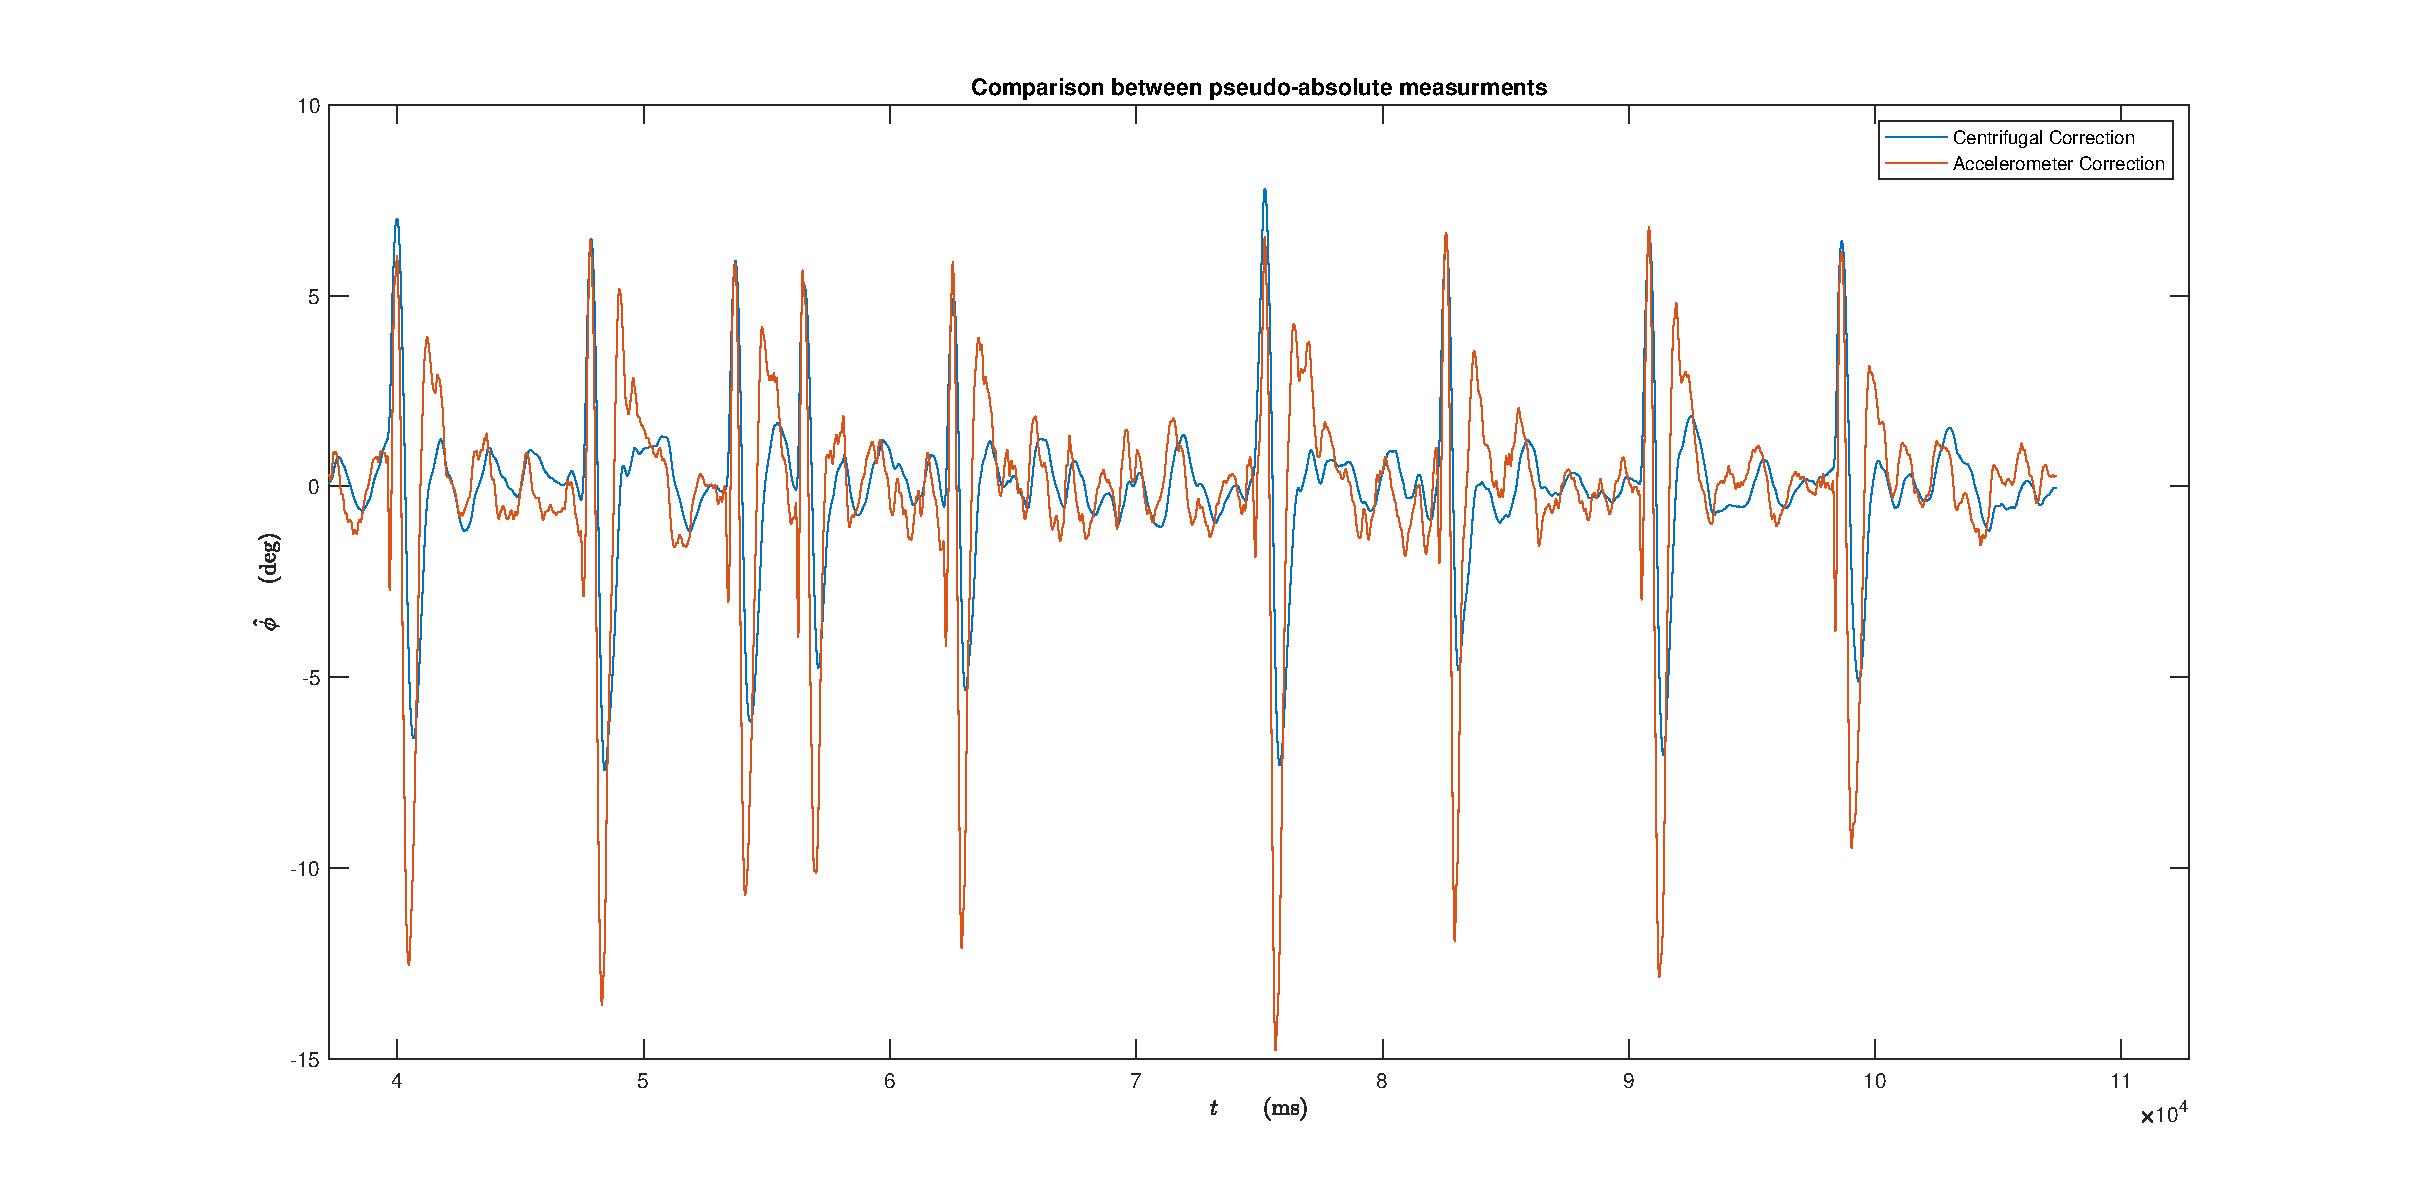
\includegraphics[width=1\linewidth]{images/figureB_1.eps}
        \caption{Comparison between pseudo-absolute measurements}
        \label{fig:results_app1}
    \end{subfigure}
    \begin{subfigure}[b]{\textwidth}
        \centering
        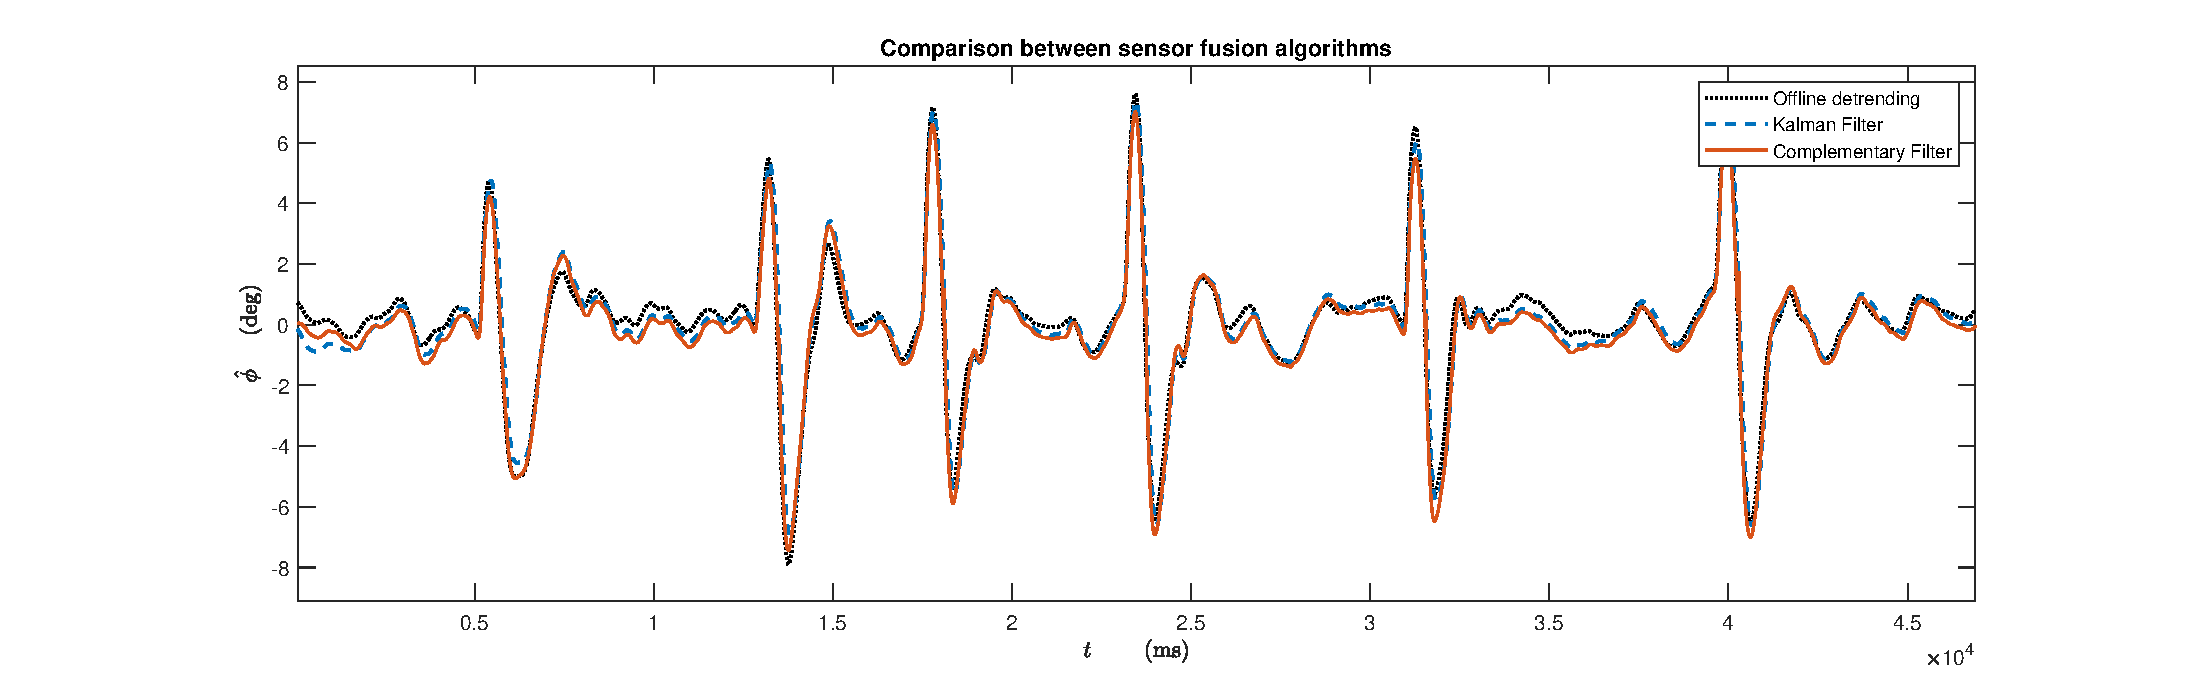
\includegraphics[width=1\linewidth]{images/figureB_2.eps}
        \caption{Comparison between sensor fusion algorithms}
        \label{fig:results_app2}
    \end{subfigure}
    \caption{a) Comparison between pseudo-absolute measurements. Both sources were fused with the integration output via a Kalman filter. The blue line is the result of the measurements used by \citet{sanjurjo2018roll} while the orange line is the result of the estimation produced using the accelerometer  \cref{eq:offset1}.b) Comparison between sensor fusion algorithms. For reference the output of the offline linear regression detrending is shown as a black dotted line.}
    \label{fig:results_app}
 \end{figure}
 
Additionally the initial covariance matrix was equal to zero which means that the filter at the start "trusts" the model output; the Euler integration output. As a reference the result from the linear regression detrending is also presented. The graph indicates that both methods successfully approximate the reference result. Furthermore, it is clear that with this general system model, only a slight performance gain (if any) can be gained by using the Kalman filter. Additionally, the implementation of the complimentary filter is far simpler and consequently much less computationally expensive. Had the Kalman filter been implemented on a system where  an accurate dynamic model was present , the Kalman filter would – in pretty much all cases – trump the simpler complimentary filter. For this reason the complimentary filter approach was chosen for the online implementation of roll estimation in the steer-by-wire bicycle, considering the limiting clock speed of microcontroller Teensy 3.6.

The above pseudo-absolute measurements can only be used to estimate the roll angle. However there is a way to extract an estimation of the yaw relative to the magnetic north by using the magnetometer sensor, which is also part of the IMU. This is similar to how modern smartphones can work as a compass. Similar to how an estimation of the roll angle was made by equating the accelerometer readings with  reference position where the gravitational acceleration is completley aligned with the bike's z-axis, the same can be done by equating the magnetometer readings with the reference position of the bike's x axis pointing towards the magnetic north. The magnetometer in this reference position are 

\begin{equation}
\boldsymbol{B}_{ref}=B\left(\begin{array}{c}{\cos \zeta} \\ {0} \\ {\sin \zeta}\end{array}\right)
\end{equation}

where B is the geomagnetic field strength and \ensuremath{\zeta} is the angle of inclination of the geomagnetic field measured downwards from horizontal. Both values vary over the earth's surface. Detailed geomagnetic field maps are available from the World Data Center for Geomagnetism at \hyperref[site]{http://wdc.kugi.kyoto-u.ac.jp/igrf/}. Fortunately, both B and \ensuremath{\zeta} cancel out in the final formulation of the estimator.


\begin{figure}[ht]
    \centering
    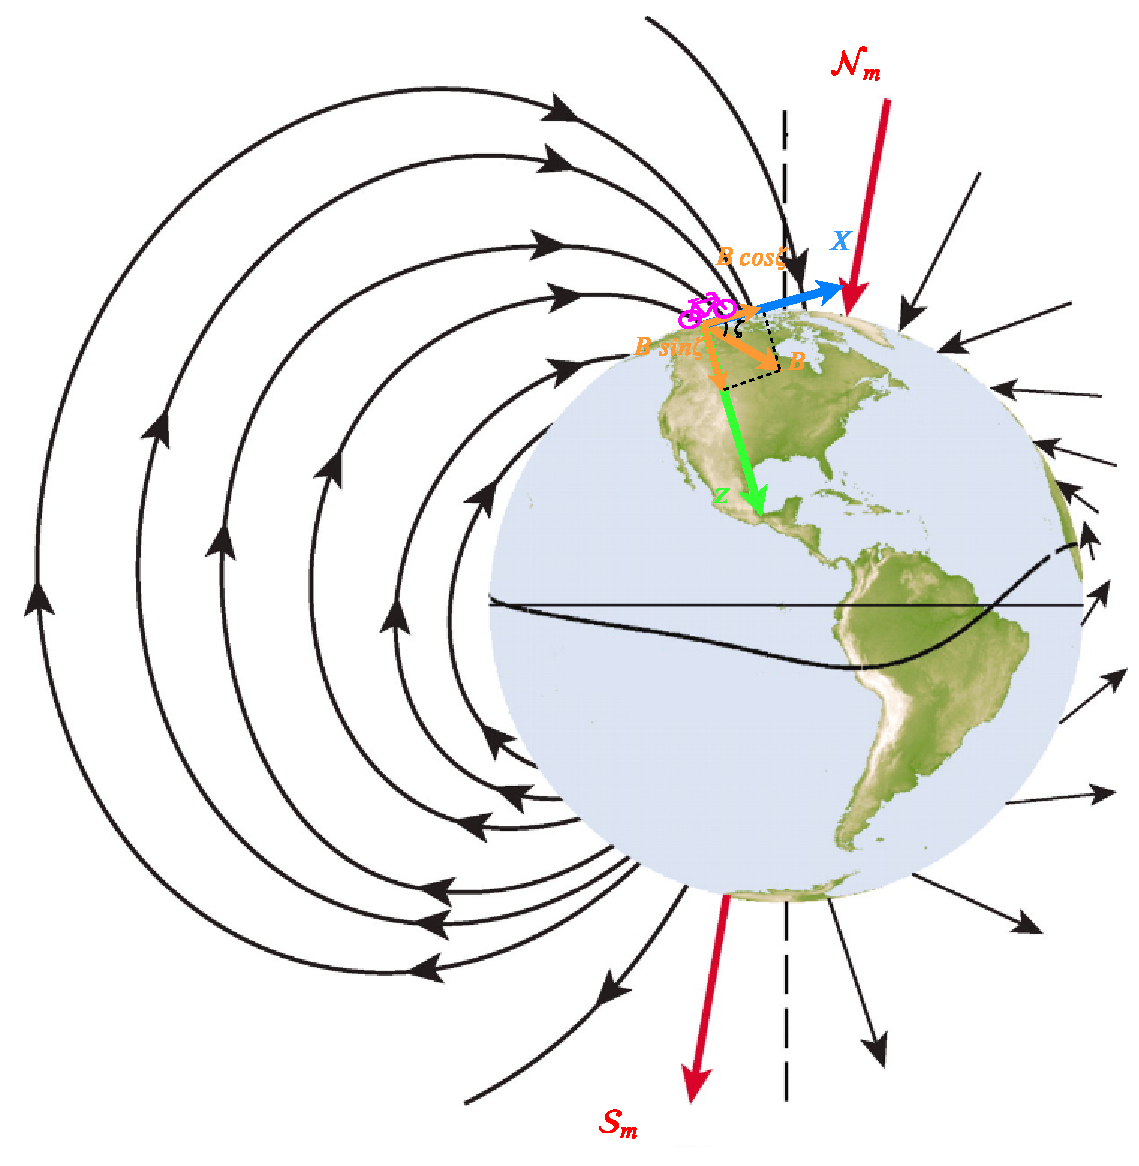
\includegraphics[scale=0.4]{images/magnetic_field_axis.pdf}
    \caption{Magnetic Field vectors in the reference position. \ensuremath{}}  
\end{figure}

The measured magnetometer readings \ensuremath{\boldsymbol{B}_{p}} after three rotations are described by equations :
\begin{equation}
    \boldsymbol{B}_{p}=\boldsymbol{R}_{\mathit{xyz}}(\phi,\theta,\psi)\cdot B\left(\begin{array}{c}{\cos \zeta} \\ {0} \\ {\sin \zeta}\end{array}\right) + \left(\begin{array}{c}{V_x} \\ {V_y} \\ {V_z}\end{array}\right)
    \label{eq:b14}
\end{equation}  

where \ensuremath{\boldsymbol{R}_{\mathit{xyz}}} the rotation matrix defined in \ref(eq:rotmat2) and \ensuremath{V_x,V_y,V_z} are the components of the Hard-Iron vector,  which is a fixed magnetic offset adding to the true magnetometer sensor output. The Hard-Iron offset is the sum of any intrinsic zero field offset within the magnetometer sensor itself plus permanent magnetic fields within the PCB generated by magnetized ferromagnetic materials. It is quite normal for the Hard-Iron offset to greatly exceed the geomagnetic field.  Therefore an accurate Hard-Iron estimation and subtraction are required.

The Hard-Iron offset can be estimated if we consider that the set of all 3d points defined by every magnetometer reading lies in the surface of a sphere with radius \ensuremath{B}. In the presense of the offset, the center of the sphere would be displaced by the Hard-Iron Vector \ensuremath{\boldsymbol{V}}. The components of vector \ensuremath{\boldsymbol{V}} can be estimated by fitting the magnetometer measurements to the equation:
\begin{equation}
    \left(\boldsymbol{B}_{p}-\boldsymbol{V}\right)^{T}\left(\boldsymbol{B}_{p}-\boldsymbol{V}\right)=B^{2}
    \label{eq:magOptim}
\end{equation}

\Cref{eq:magOptim} was solved with the gradient descend method by minimizing the  sum of the squared difference between the right and left hand side of the equation. The resulting Hard-Iron Offset Vecotor was :

\begin{equation}
    \boldsymbol{V}=\left(\begin{array}{ccc} -22.03 & -26.14 & -1.651 \end{array}\right)\;\;\;\;\;\;\;\;\;\;[\si{\micro\tesla}]
\end{equation}

In \cref{fig:sphere_mag} the locus defined by the set of vectors measured by the magnetometer is displayed. It is visible that after the correction the measurements lie on the surface of a sphere with center in the origin and radius approximately equal to 1 a.u.

\begin{figure}[ht]
    \centering
    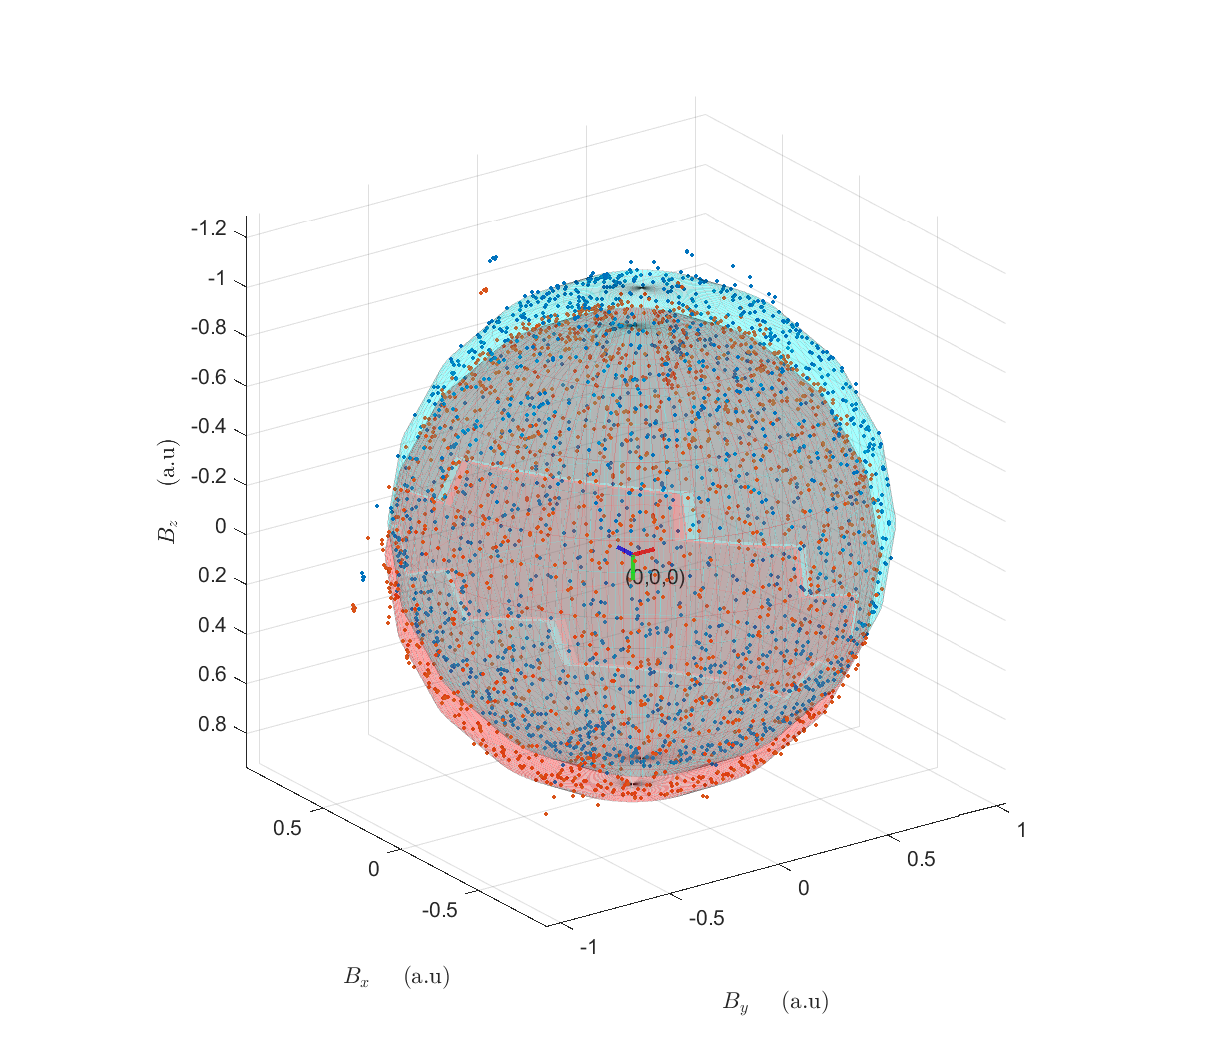
\includegraphics[scale=0.5]{images/magnet_sphere.eps}
    \caption{The blue dots are the locus of the magnetometer readings before correcting for the hard iron offset. The red dots are the locus of the magnetometer readings after correcting for the offset. The magnetometer readings have been normalized so that 1 a.u\ensuremath{=49.0913\; \si{\micro\tesla}} which is the Magnetic Field Intensity for the approximate location of TU Delft (Latidude  52\si{\degree} 0' 0" N and Longitude: 4\si{\degree} 22' 0" E).}
        \label{fig:sphere_mag}
\end{figure}

Having estimated \ensuremath{\boldsymbol{V}} from \cref{eq:b14} by assuming \ensuremath{\theta\approx0} we get :



\begin{align}
    \boldsymbol{B}_f = \boldsymbol{B}_p-\boldsymbol{V} &= \boldsymbol{R}_x(\phi)\boldsymbol{R}_z(\psi)\cdot \left(\begin{array}{c}{B\cos \zeta} \\ {0} \\ {B\sin \zeta}\end{array}\right)  \\
    \boldsymbol{R}^T_x(\phi)\left(\begin{array}{c}{B_{fx}} \\ {B_{fy}} \\ {B_{fz}}\end{array}\right)   &= \left(\begin{array}{c}{\cos \psi B \cos \delta} \\ {-\sin \psi B \cos \delta} \\ {B \sin \delta}\end{array}\right) \\
    \left(\begin{array}{c}{B_{f x} } \\ {B_{f y} \cos \phi-B_{f z} \sin \phi} \\ {B_{f y} \sin \phi+ B_{f z}  \cos \phi}\end{array}\right) &= \left(\begin{array}{c}{\cos \psi B \cos \delta} \\ {-\sin \psi B \cos \delta} \\ {B \sin \delta}\end{array}\right) \label{eq:B18}
\end{align}

By dividing the y and x component of  \cref{eq:B18} we get:
\begin{equation}
    \hat{\psi}=tan^{-1}\left(\frac{B_{f z}sin\hat{\phi}-B_{f y}cos\hat{\phi}}{B_{f x}}\right)
    \label{eq:psiMag}
\end{equation} 

where \ensuremath{\hat{\phi}} is the estimate of roll angle obtained from the aforementioned methods. \Cref{eq:psiMag} can now be used as a source of pseudo-absolute measurements for the sensor fusion algorithm of choice. Regarding signal fusion the same things apply as in the roll angle estimation case. Finally since we want the yaw angle relative to the starting position and not relative to the magnetic north the value of the first yaw estimation is subtracted from all subsequent computations.

\begin{figure}
    \centering
    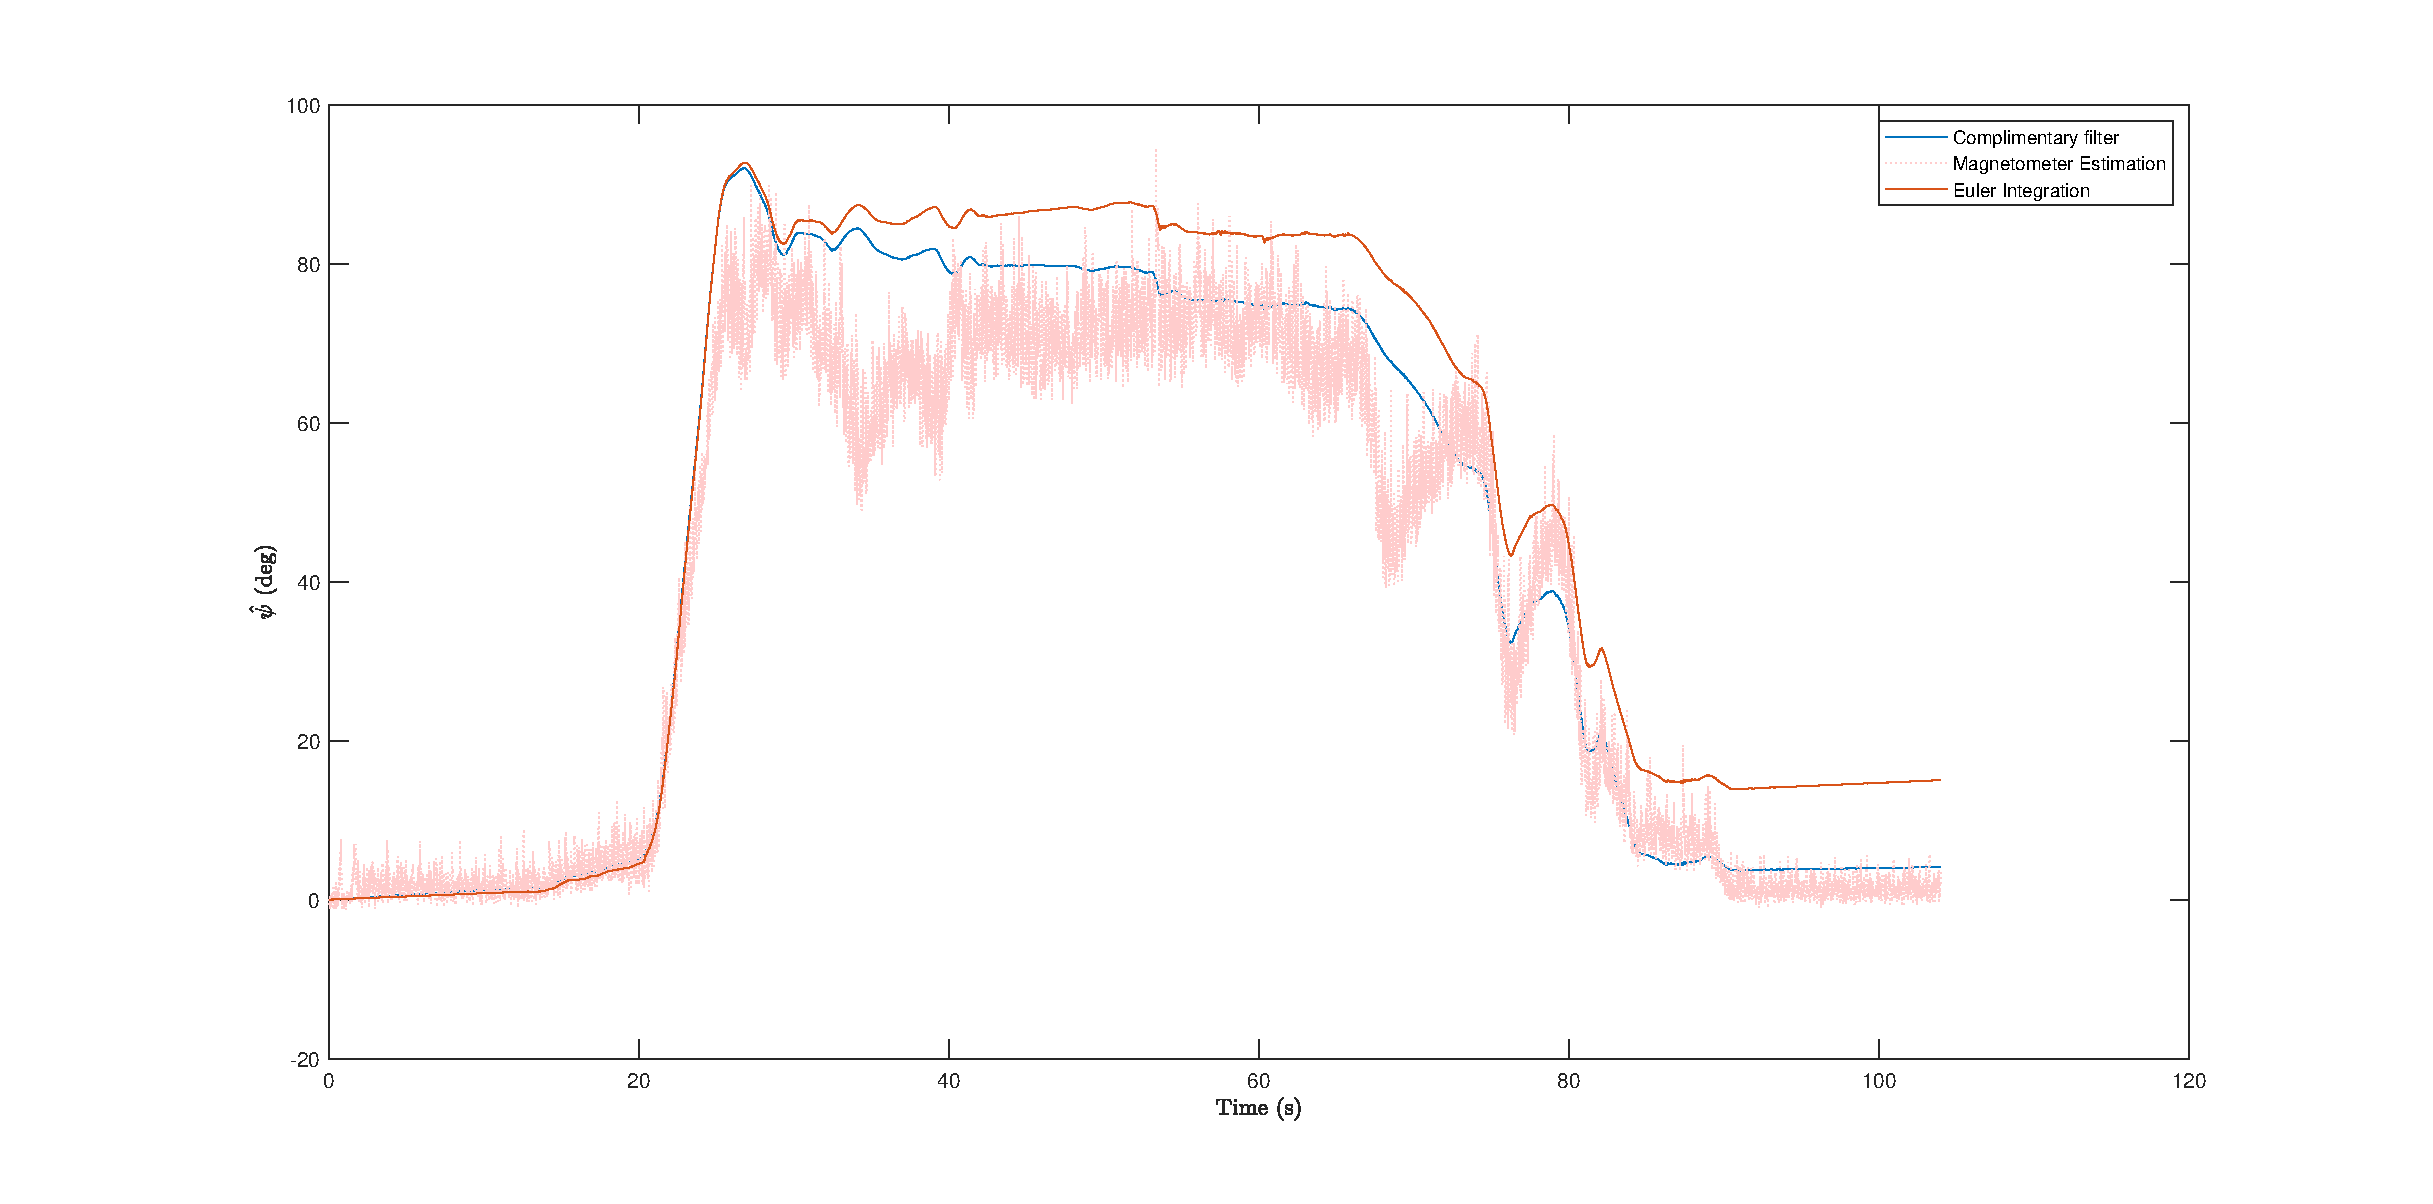
\includegraphics[width=\textwidth]{images/figureB_3.eps}
    \caption{Comparison of online yaw angle estimation.Red dotted line is the pure estimation from the magnetometer data. Orange line is the drifted euler integration output. Blue line is the result of the complimentary filter sensor fusing the other two signals. For the complimentary filter \ensuremath{a=0.00027}.}
\end{figure}